\section{Compute Engine}\label{sec:design}

The computing engine, which is most fundamental part, is based on the QuantLib\cite{quantlib}. We define new \textbf{instrument classes} if not exist in QuantLib. The instruments include the Equity Swap and Cross Currency Swap mentioned in Section~\ref{sec:scope}, also BVA and TVA which is treated as prices. We create new \textbf{pricing engines} for existing and new instruments, including ones using analytical solutions and Monte Carlo methods. Computation of exposure at default time for specific instruments is isolated into \textbf{instrument models} and \textbf{counterparty models}.

\begin{figure}[h]
  \centering
  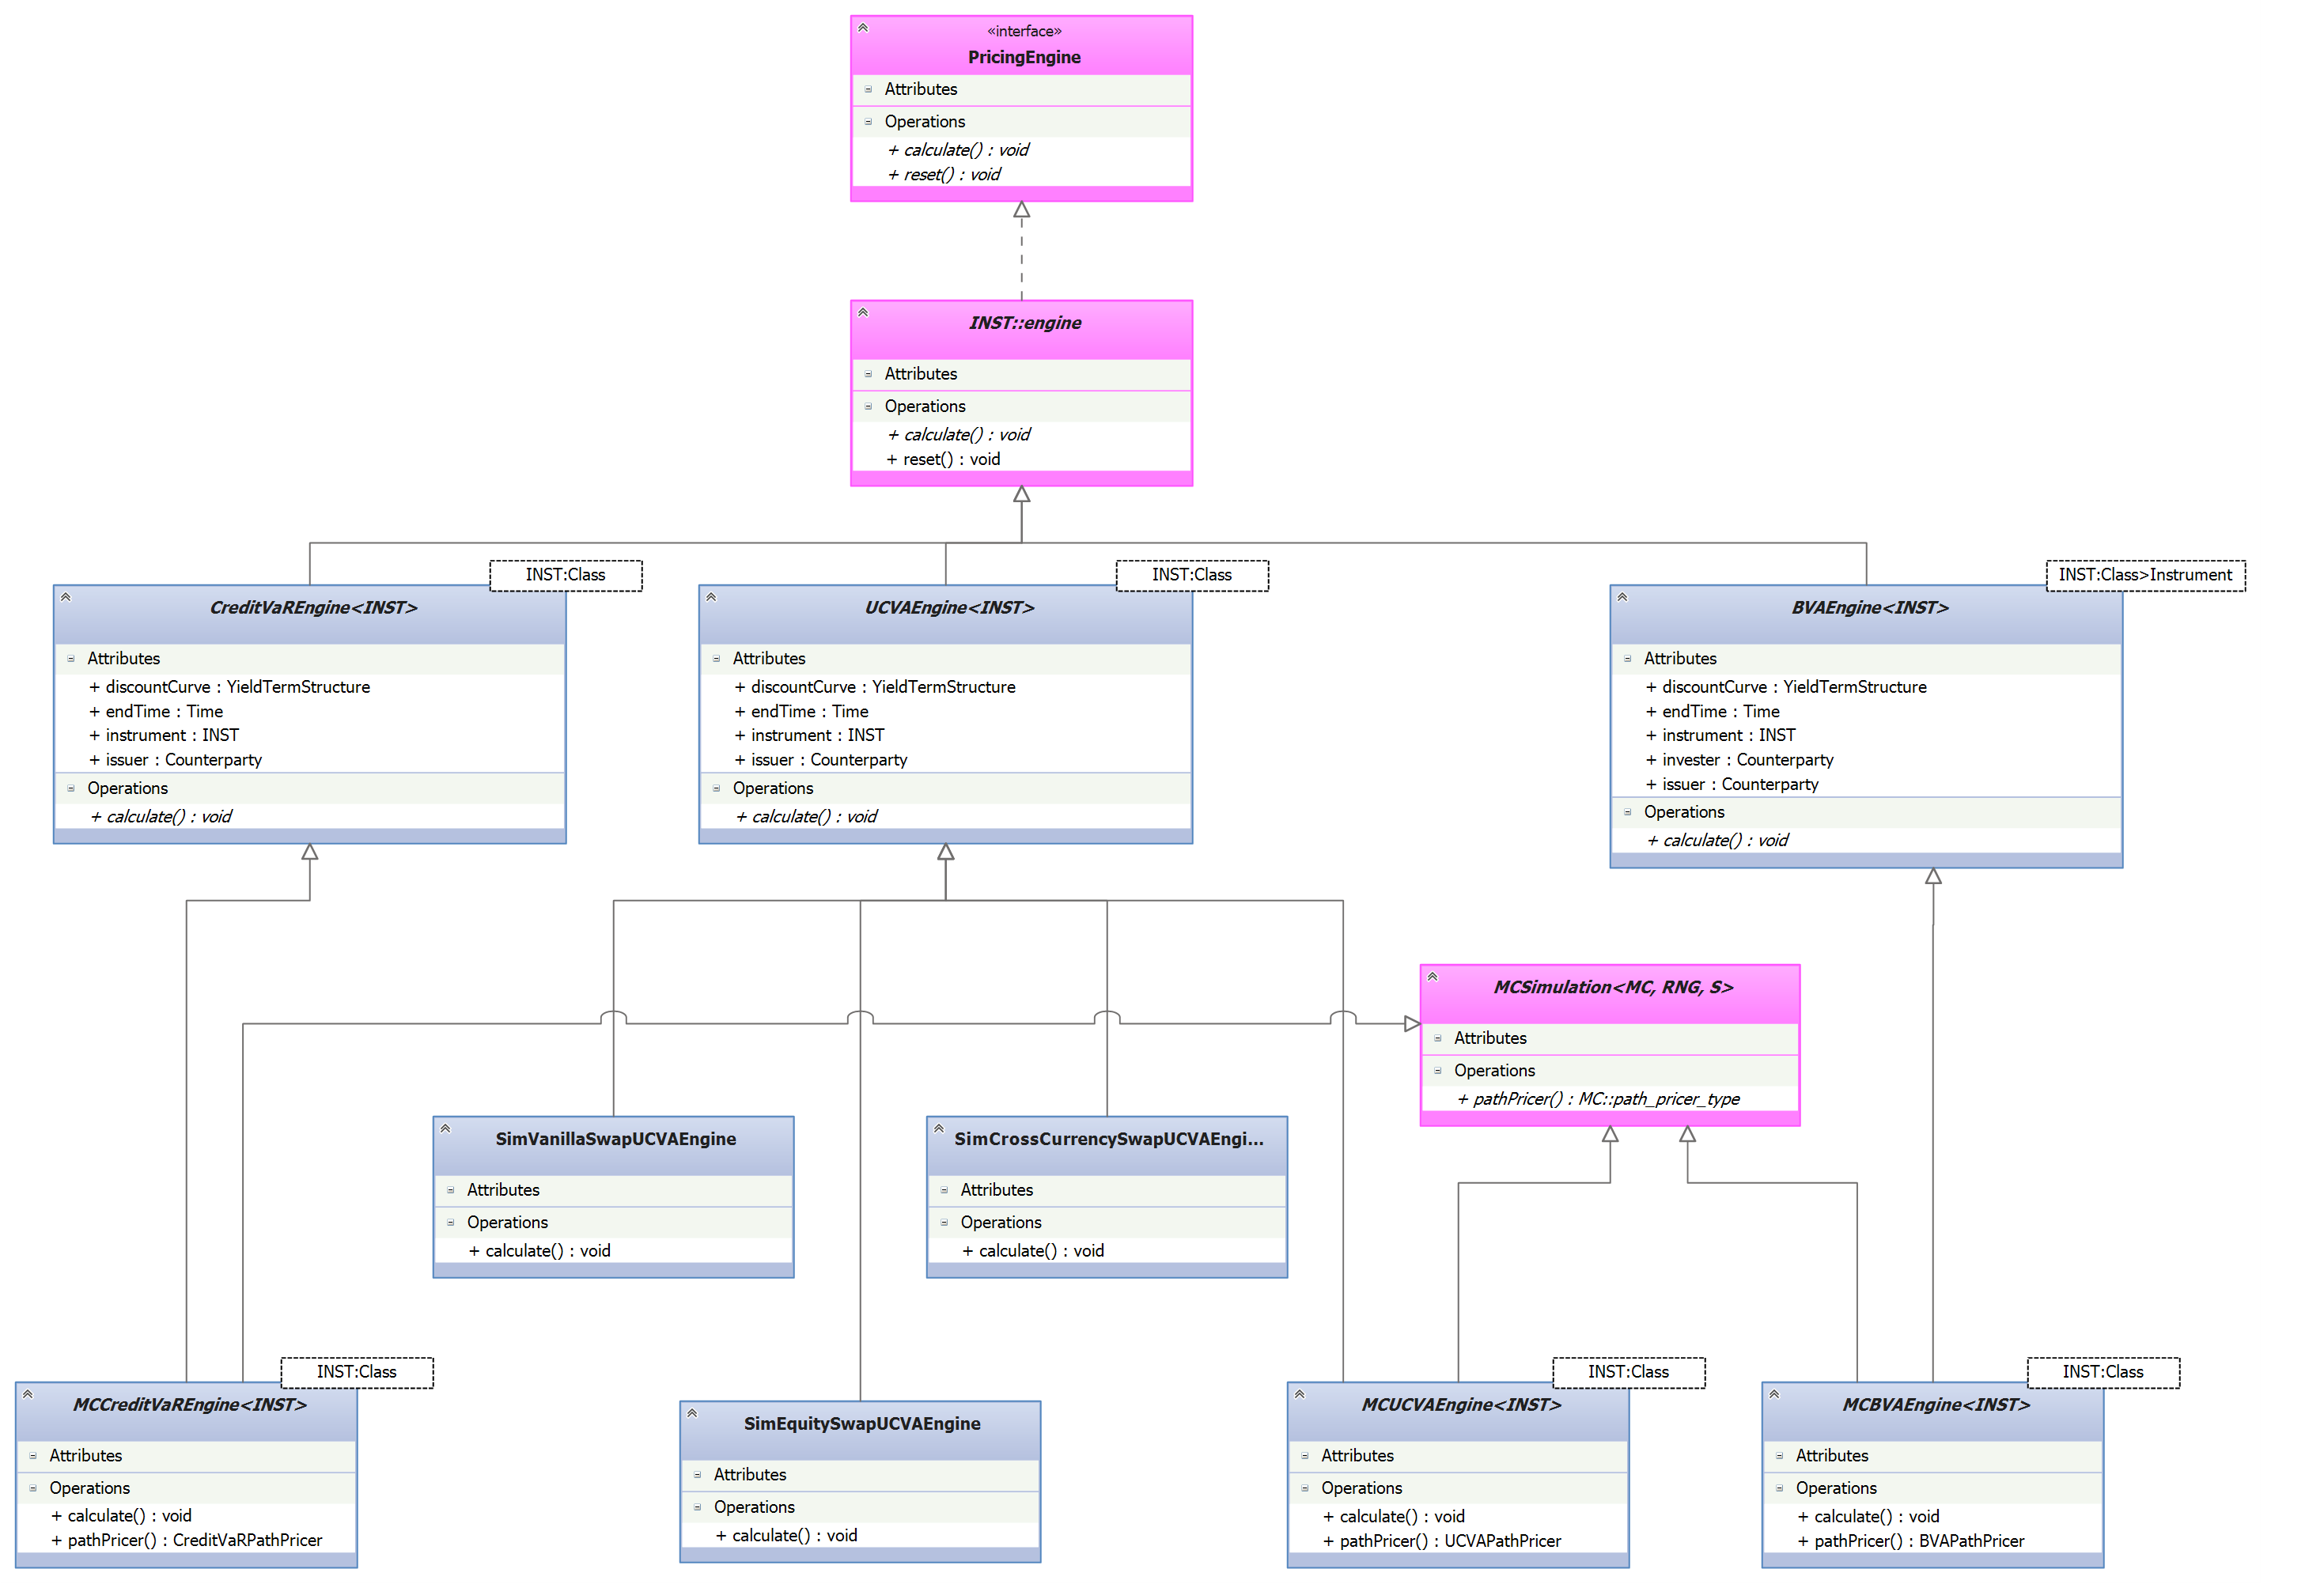
\includegraphics[width=0.8\textwidth]{pricingengine.png}
  \caption{Pricing Engines}\label{fig:pricingengines}
\end{figure}

\subsection{Default Models and Counterparties}

\begin{figure}
  \centering
  \subfigure[Default Models]{\label{fig:defaultmodel}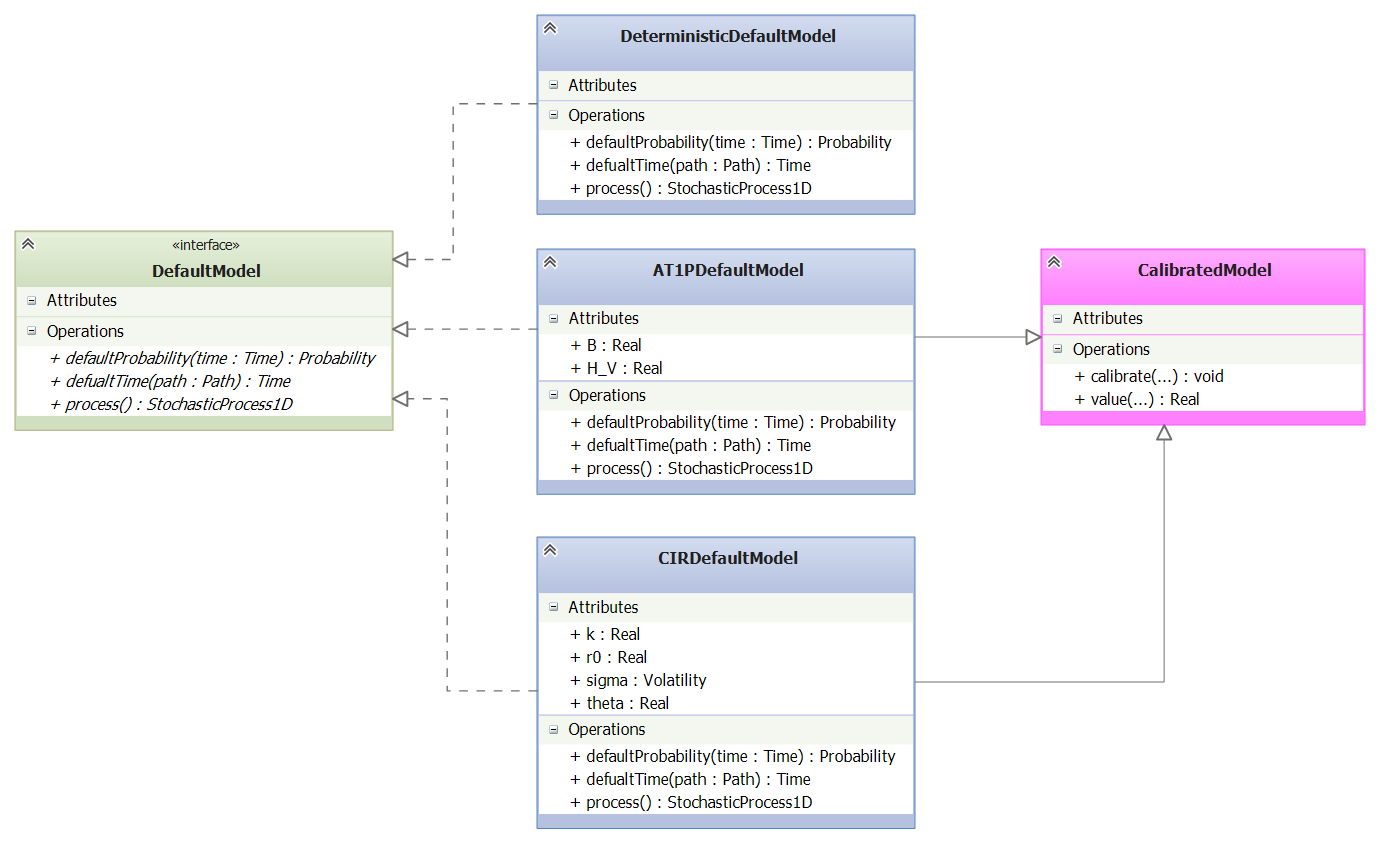
\includegraphics[width=0.6\textwidth]{defaultmodel}}
  ~~~~
  \subfigure[Counterparties]{\label{fig:counterparty}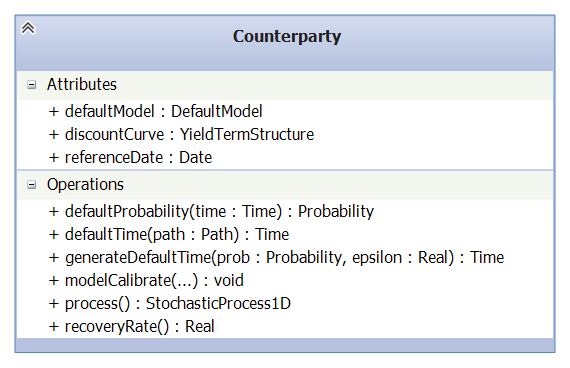
\includegraphics[width=0.3\textwidth]{counterparty}}
  \caption{Default and Counterparty Models}\label{fig:defaultandcouterparties}
\end{figure}

Default models usually require calibration using market data. As a result, we implement the default model using the calibrated model framework in QuantLib. The Counterparty class, which will be used by the BVA and TVA engine, will hold a reference to a specific default model. In addition, the counterparty object have information of recovery rate and default time information related to the counterparty risk. The class diagrams of default models and counterparty are shown in Figure~\ref{fig:defaultmodel} and Figure~\ref{fig:counterparty}.

The \textbf{Analytically-Tractable First Passage (AT1P) Model}~\cite{brigobook}, which is a firm value (or structural) model, assumes the risk neutral dynamics for the value of the firm $V$ is characterized by a risk-free rate $r_t$, a payout ratio $k_t$ and an instantaneous volatility $\sigma_t$, according to the equation:
$$ dV_t=V_t(r_t-k_t)dt + V_t \sigma_t dW_t $$
and assume a default barrier $H(t)$ of the form 
$$H(t) = H exp(\int_0^t (r_u-k_u-B \sigma_u^2) du )$$
where H and B are parameters.

The \textbf{Cox-Ingersoll-Ross (CIR) Model}, which is a intensity model that modelling default intensity using short-rates, assumes
$$dr_t = k(\theta-r_t)dt + \sigma \sqrt{r_t} dW_t $$
where
$$2k\theta > \sigma^2 $$


\subsection{General Monte Carlo Engines}

For computation of BVA and TVA using Monte Carlo, the only part depend on the specific instrument is the exposure and underlying process, as a result, we externalize the exposure computation into underlying model, the counterparty default modelling to the counterparty and default model, and leave other parts to a shared Monte Carlo engine. For example, recall the computation of bilateral CVA, DVA and FVA

$$ CVA=\mathbb{E}_0^Q[(1-REC)D(0,\tau)\mathbf{1}_{\{\tau_{1st}=\tau_C<T\}}Ex(\tau)^+] $$

$$ DVA=\mathbb{E}_0^Q[(1-REC)D(0,\tau)\mathbf{1}_{\{\tau_{1st}=\tau_I<T\}}Ex(\tau)^-] $$

$$ FVA=-\mathbb{E}_0^Q[\int_0^T{1_{\{\tau_{1st}>t\}} D(0,t) \gamma(t)(V(t,T)^+ + V(t,T)^-)} dt]$$

The counterparty provides the recovery rate and determines which counterparty defaults (if any), and the Monte Carlo BVA engine handle all the computing workflow, such as discounting, checking first-to-default condition, and taking the expectation of all paths. The only instrument-specific part is the computation of exposure $Ex(\tau)$. The class diagram of Monte Carlo exposure models are shown in Figure~\ref{fig:mcexposure}

\begin{figure}[h]
  \centering
  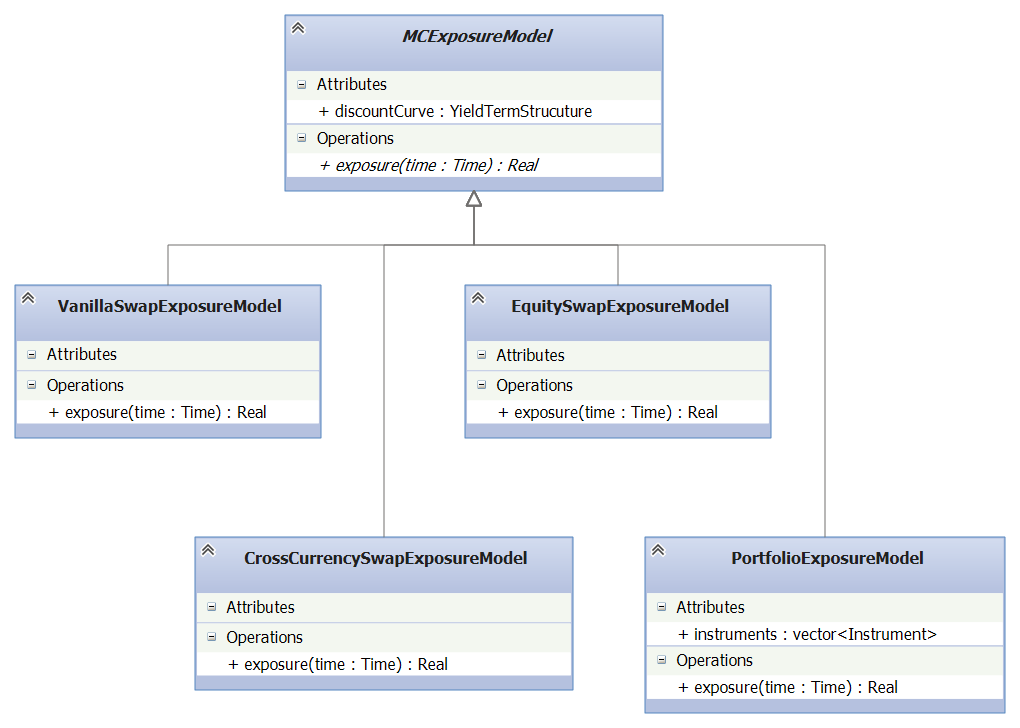
\includegraphics[width=0.6\textwidth]{mcexposure.png}
  \caption{MC Exposure Models}
  \label{fig:mcexposure}
\end{figure}

By externalizing the instrument-specific parts, we are also able to support computing the BVA and FVA for a portfolio rather than just a single position. Specifically, the general Monte Carlo engine simulates the underlying processes with correlation in consideration, then for each path, it invokes the instrument model separately to get the exposure for each single instrument. After getting all the single instrument exposures, it aggregate them according to the netting rules. Then the other parts of the computing the BVA and FVA are not affected.

\subsection{Instrument-Specific Unilateral CVA Engines}

For some simple cases, it's possible that we can compute the CVA, DVA and/or FVA without full Monte Carlo simulation. In our project, we implement the unilateral CVA engine for single instruments supporting IRS, Equity Swap and CCS, without Wrong Way Risk. In case that the the portfolio contains a single instrument and no Wrong Way Risk is required, we can use analytic or synthetic solution to get the unilateral CVA efficiently. The method we compute the unilateral CVA is from \cite{brigobook}. 
